
\section{Task B}
The agent is an object with a finite set of rules that will move around the
environment.  Our simple reflex agent requires the assumption that the
environment is a rectangular shape, surrounded by walls and free of obstacles.

We've also contemplated an algorithm that will recursively move around the
environment and mark the visited cells to avoid an endless loop situation.

The problem with the recursive algorithm is that the agent has to manage the
counters and initiate the performance calculation itself.

\subsection{Agent}
The agent has the following attributes, some are not used during the algorithms
but will be needed for other types of algorithmic designs. See figure
\ref{fig:agent_uml} for the uml description of bot attributes and functions.

\begin{figure}[h] \label{fig:agent_uml}	\centering
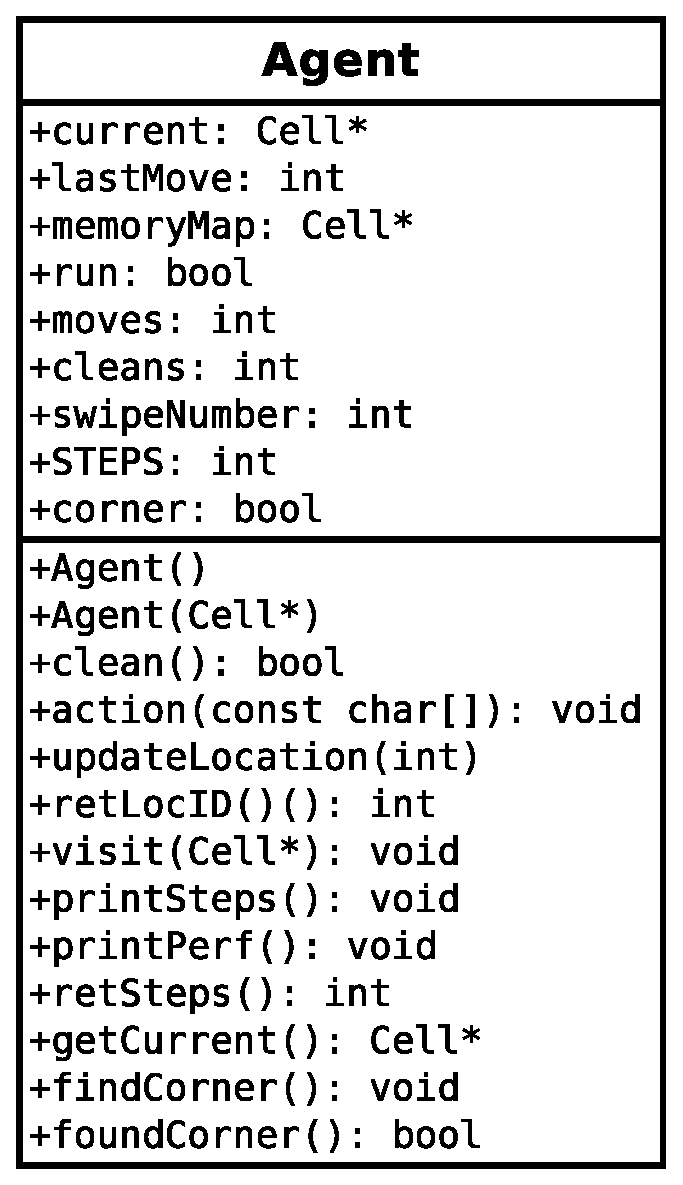
\includegraphics[width=0.3\textwidth]{agent_um}
\caption{UML description of an Agent object}
\end{figure}

\begin{description}
\item[current:]
	This is a Cell* pointer which will point to the current location of the agent.
	Whenever the agent moves the "current" attribute has to be changed to point to
	the new Cell object, which is done by calling the current locations getNeighbor
	function which returns the Cell* pointer to its neighbor.
\item[lasMove:]
	This is an integer describing the direction of the last move made. The moves
	possible are described as a global ENUM as "LEFT", "RIGHT", "UP" and "DOWN".
	By utilizing this the agent can avoid going back to its previous location,
	unless nessecary
\item[memoryMap:]
	This is not currently in use, but can be used to start building a map of the
	environment inside the robots head.  This is set as a Cell, but should be made
	into a different object type with minimal information.
\item[run:]
	This is a boolean value which could  be used to make the agent power down and
	stop cleaning/moving.  Which could be usefull if the room will never get dirtu
	again, since it could stop when finding the second corner.
\item[moves:]
	This is a counter which counts how many movements the agent has performed
	during its run.  This is used when displaying the performance rate of the
	agent.
\item[cleans:]
	This is a counter of how many cells the agent has cleaned during its run. The
	attribute is used during display of the performance rate.
\item[swipeNumber:]
	This is an integer that describes which way the agent is supposed to move.
	The agent will increment this counter each time it hits a wall and thereby
	switch moving to a side. 
\item[STEPS:]
	This is an internal counter to count the number of times the agent has
	perfomed an operation and is used to stop the agent after a certain amount of
	operations.  The counter is for creating an equal amount of movements during
	performance testing.
\item[corner:]
	This is an boolean value describing whether or not the corner has been found.
	The value is set to false during initation and true when the corner is found.
	By utilizing this we can switch from performing the find  corner algorithm to
	our movement algorithm.
\end{description}

\subsection{Simple algorithm}


\begin{figure}[h] \label{fig:corner}	\centering
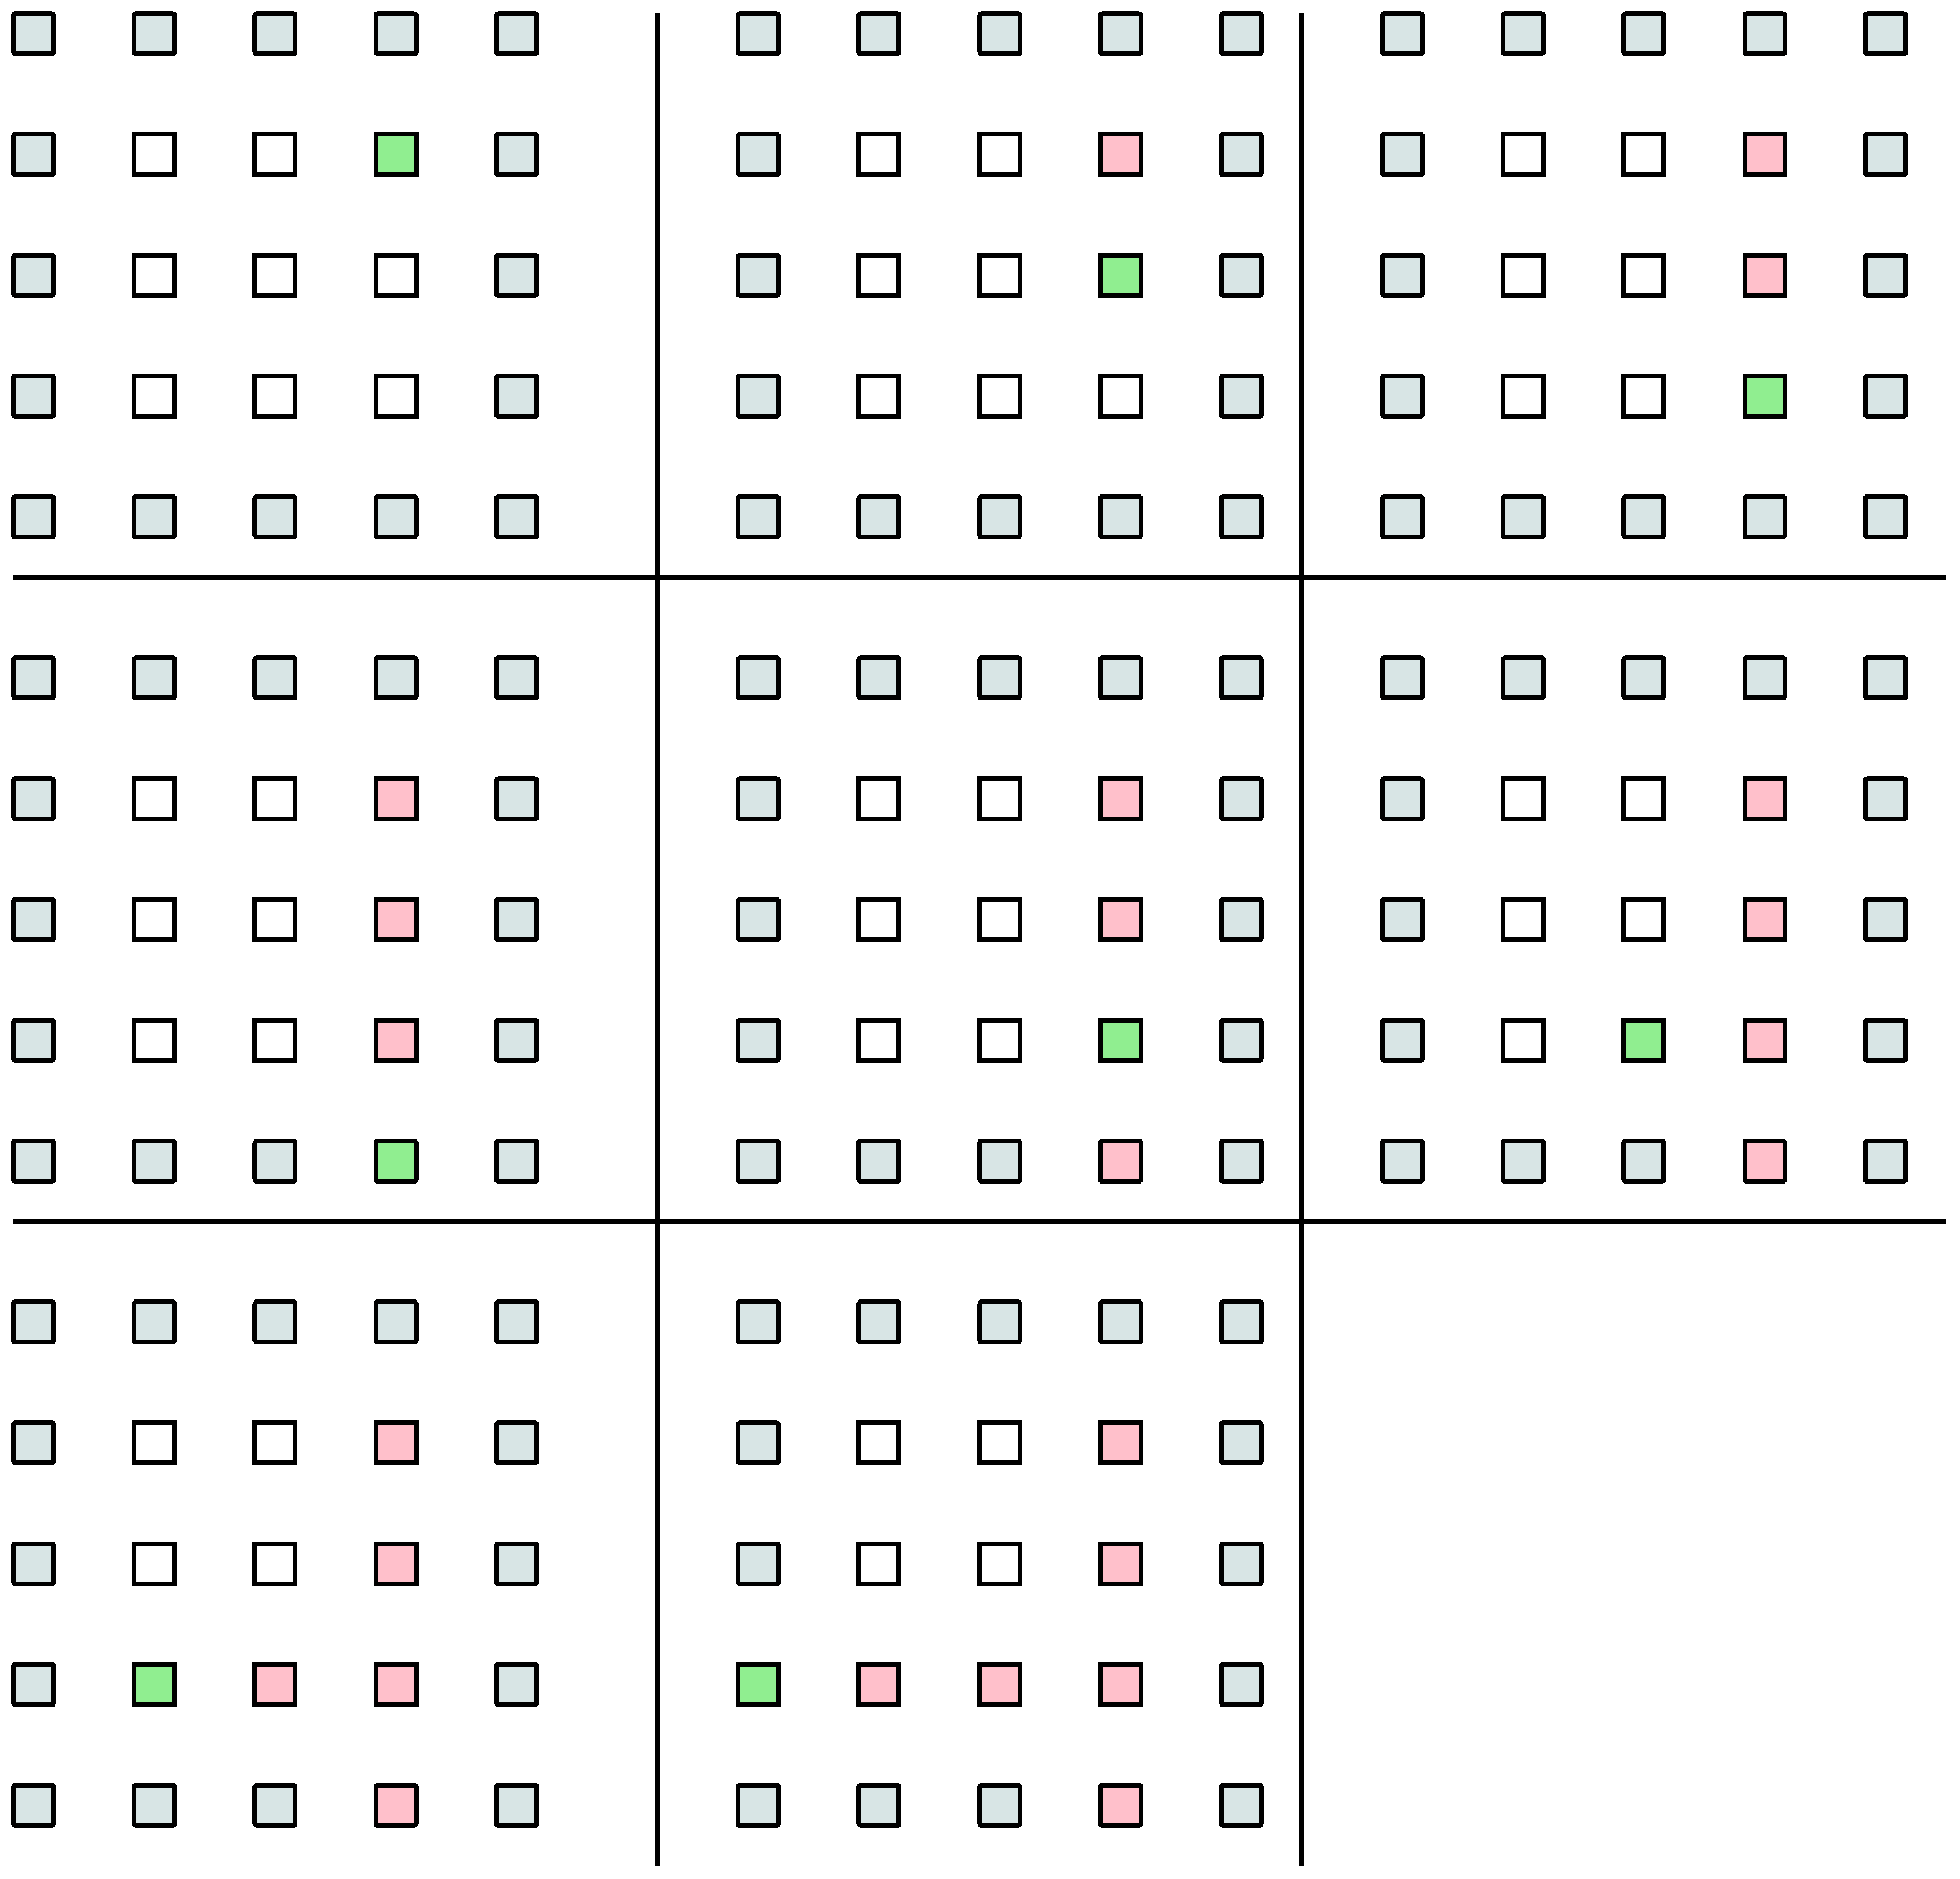
\includegraphics[width=0.5\textwidth]{find_corner}
\caption{How the agent finds the corner}
\end{figure}


\subsection{Harder algorithm}


\begin{figure}[h] \label{fig:}	\centering
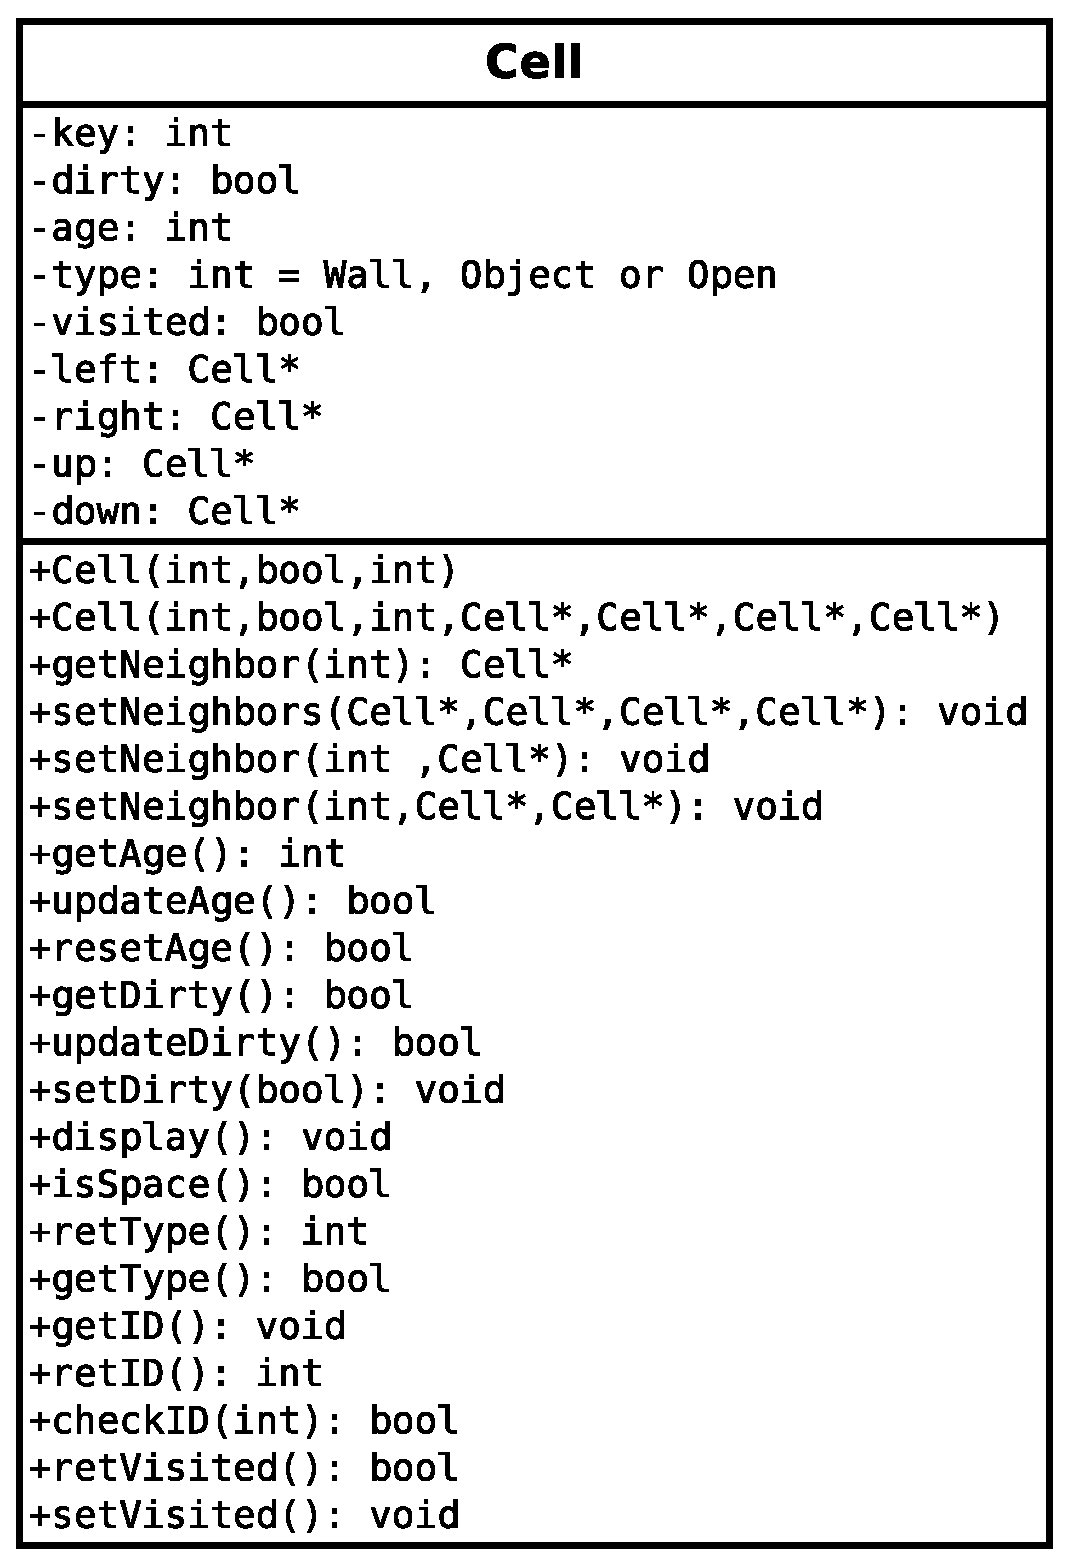
\includegraphics[width=0.3\textwidth]{cell_uml}
\caption{}
\end{figure}

\begin{figure}[h] \label{fig:}	\centering
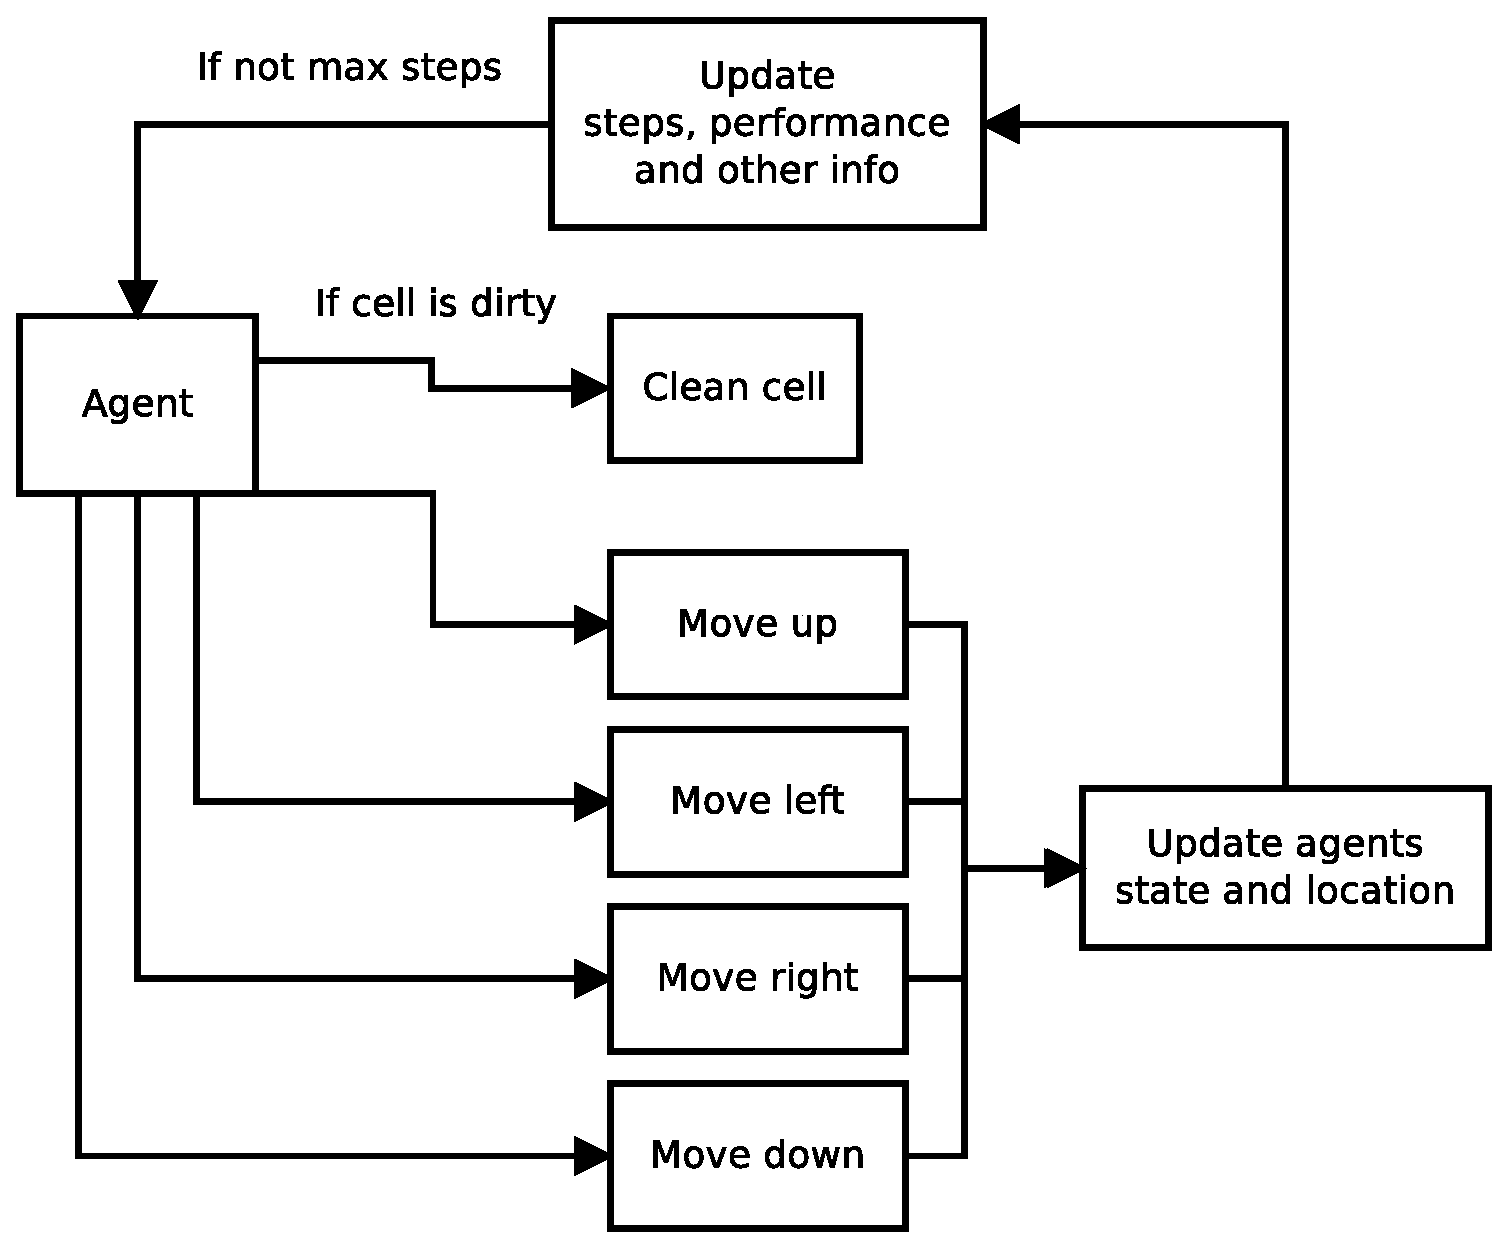
\includegraphics[width=0.5\textwidth]{agent}
\caption{}
\end{figure}




